\begin{figure}[ht]
    \centering
    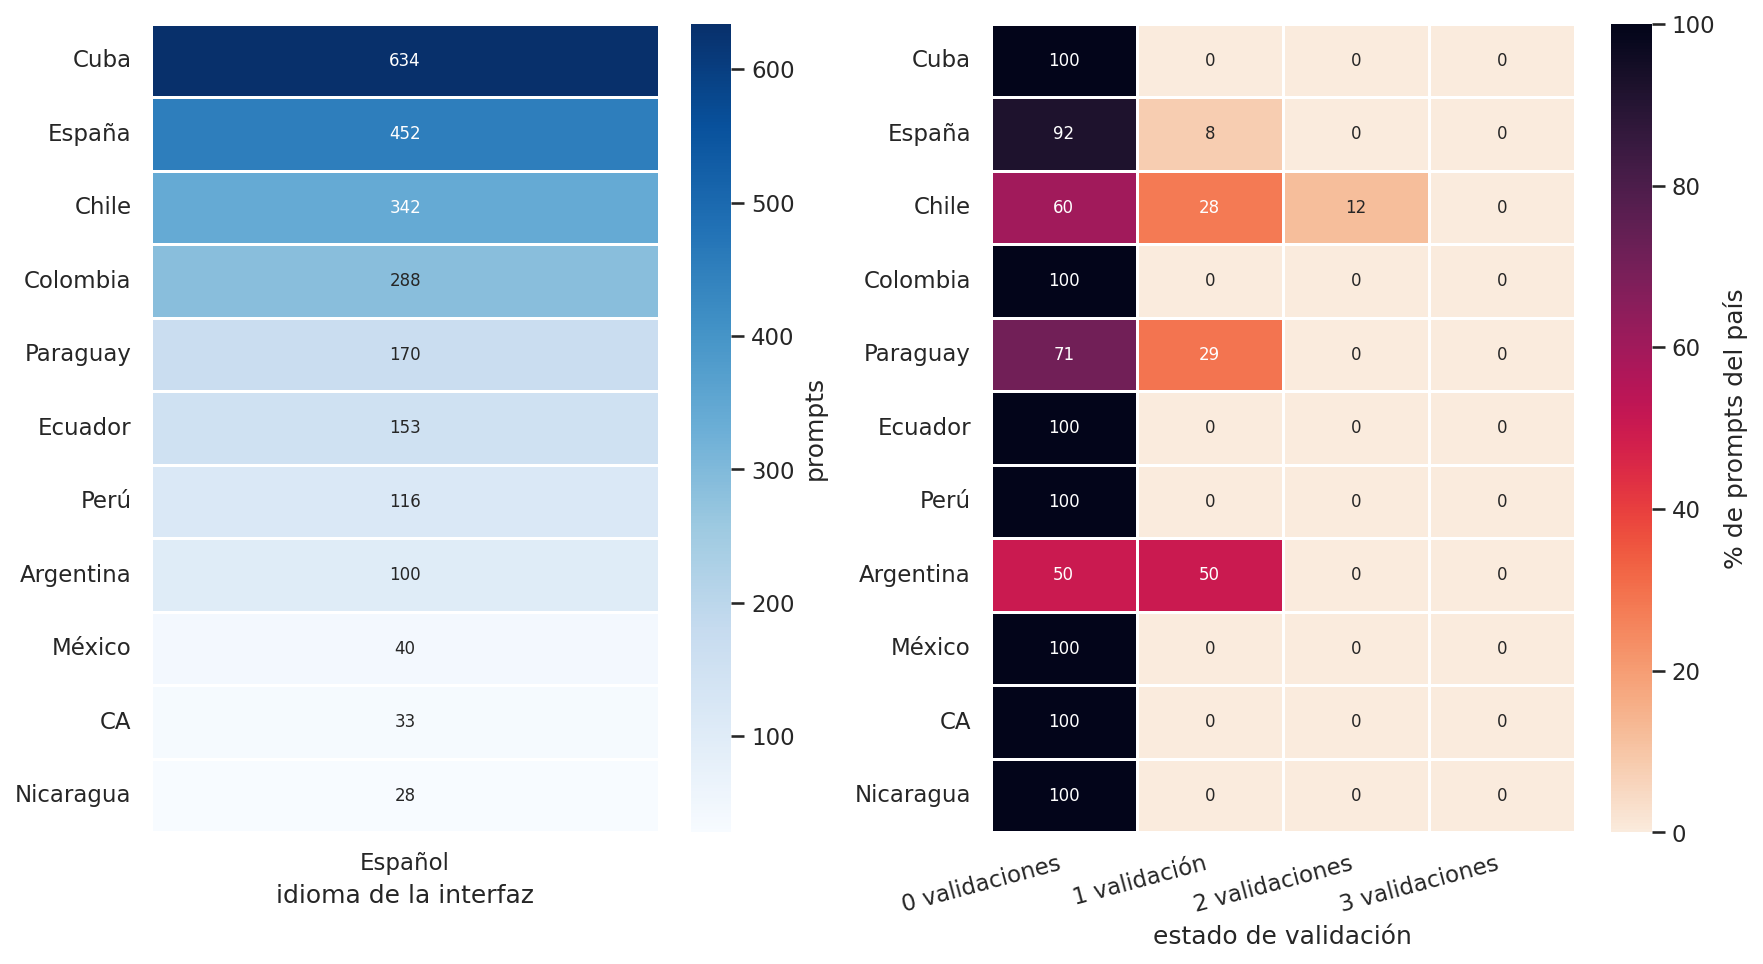
\includegraphics[width=0.95\textwidth]{mapa_pais_idioma_estado.png}
    \caption{Estado del pipeline por país. Panel izquierdo: número absoluto de prompts por país, segmentado por idioma de la interfaz; el color saturado señala los países con más volumen. Panel derecho: distribución porcentual del estado de validación dentro de cada país (qué porcentaje tiene 0, 1, 2 o 3 validaciones registradas); el color saturado marca dónde se acumulan prompts sin tocar y dónde se completan los tres slots. Combinados, ambos paneles muestran al organizador dónde tiene volumen pero falta validación, y dónde le falta volumen sin más.}
    \label{fig:mapa_pais_idioma_estado}
\end{figure}
